\documentclass[tikz,border=5pt]{standalone}
\usepackage{fontspec}\setmainfont{Latin Modern Roman}
\usetikzlibrary{positioning,arrows.meta,fit}
\begin{document}
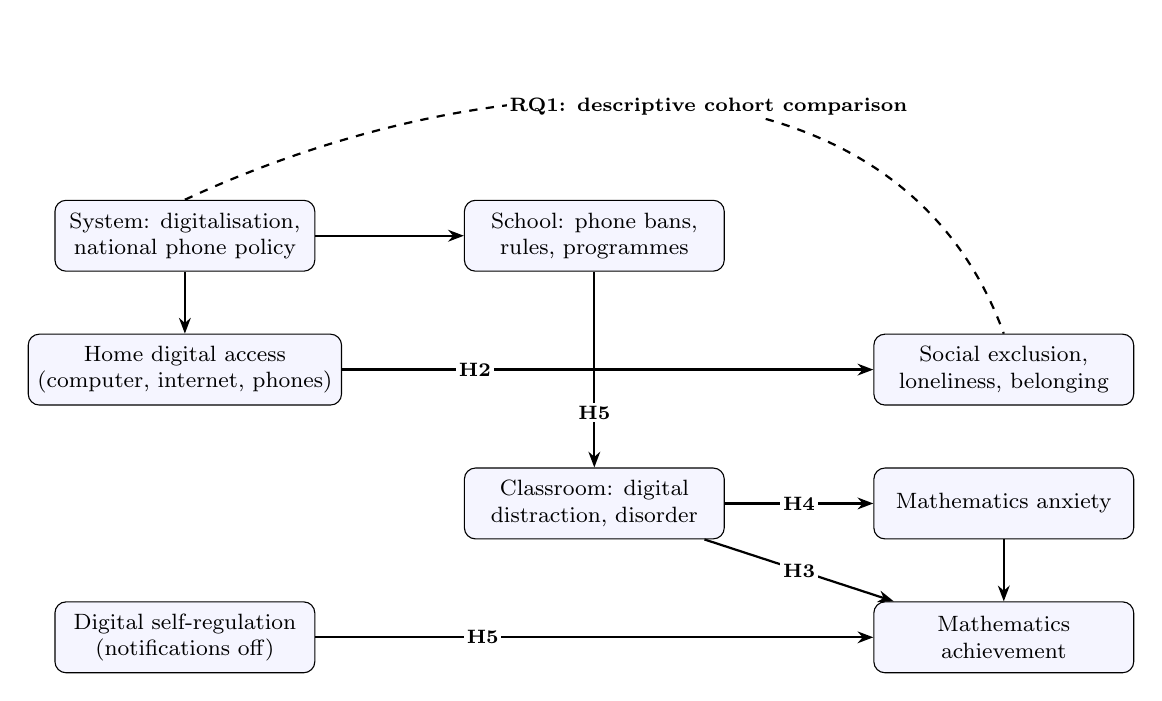
\begin{tikzpicture}[every node/.style={font=\footnotesize, align=center},
  box/.style={draw, rounded corners, minimum width=33mm, minimum height=9mm, fill=blue!4},
  arr/.style={-{Stealth[length=2mm]}, thick}, lab/.style={font=\scriptsize\bfseries, fill=white, inner sep=1pt}]
\node[box] (sys) at (0,0) {System: digitalisation,\\national phone policy};
\node[box] (sch) at (5.2,0) {School: phone bans,\\rules, programmes};
\node[box] (home) at (0,-1.7) {Home digital access\\(computer, internet, phones)};
\node[box] (wb) at (10.4,-1.7) {Social exclusion,\\loneliness, belonging};
\node[box] (class) at (5.2,-3.4) {Classroom: digital\\distraction, disorder};
\node[box] (anx) at (10.4,-3.4) {Mathematics anxiety};
\node[box] (self) at (0,-5.1) {Digital self-regulation\\(notifications off)};
\node[box] (ach) at (10.4,-5.1) {Mathematics\\achievement};
\draw[arr] (sys) -- (home);
\draw[arr] (sys) -- (sch);
\draw[arr] (home) -- node[lab, pos=.25]{H2} (wb);
\draw[arr] (sch) -- node[lab, pos=.72]{H5} (class);
\draw[arr] (class) -- node[lab]{H4} (anx);
\draw[arr] (class) -- node[lab]{H3} (ach);
\draw[arr] (anx) -- (ach);
\draw[arr] (self) -- node[lab, pos=.3]{H5} (ach);
\draw[thick, dashed] (sys.north) to[out=25, in=110] node[lab, pos=.55]{RQ1: descriptive cohort comparison} (wb.north);
\end{tikzpicture}
\end{document}